%*****************************************************************************************
%*********************************** Fifth Chapter **************************************
%*****************************************************************************************

\chapter{Micromechanical exfoliation of lead iodide perovskites}

\graphicspath{{Chapter5/Figures/}}

\nomenclature[z-CHPI]{CHPI}{\ce{(C6H9C2H4NH3)2PbI4}}
\nomenclature[z-C$_{12}$PI]{C$_{12}$PI}{\ce{(C12H25NH3)2PbI4}}
\nomenclature[z-MWQ]{MQW}{Multiple quantum well}
\nomenclature[z-BF]{BF}{Bright field}
\nomenclature[z-DF]{DF}{Dark field}
\nomenclature[z-AFM]{AFM}{Atomic force microscope}
\nomenclature[z-SPP]{SPP}{Surface plasmon polariton}
\nomenclature[z-LSP]{LSP}{Localised surface plasmon}
\nomenclature[z-SEM]{SEM}{Scanning electron microscope}

\section{Introduction}
Uniform thin films of PbI perovskites can be created over large areas as a result of spin coating, however it is hard to achieve thicknesses $\lesssim20$\,nm. For thinner samples a layer-by-layer deposition technique can be used \cite{Era2000, Matsui2002}. Micromechanical exfoliation is another way of producing ultra-thin samples, where thicker crystals are cleaved to form progressively thinner samples.

In recent years much attention has been paid to 2D layered compounds such as graphene or transition metal dichalcogenides. Due to weak van der Waals bonding, it is easy to separate neighbouring layers and form ultra-thin samples \cite{Novoselov2004, Blake2007, Ni2007, Splendiani2010, Castellanos-Gomez2010, Tonndorf2013}. In these materials new optical and electronic properties emerge for mono- or few-layer regions, providing new avenues for material application. In this Chapter I report the micromechanical exfoliation of 2D PbI perovskites, and explore the few-layer behaviour of such systems via optical spectroscopy.

\section{Experimental methods}
Prepartion of exfoliated PbI perovskite samples is shown in Fig.\,\ref{5Fig1}. Lead iodide (\ce{PbI2}) microcrystals are synthesized using a previously described solvothermal method, and intercalated using an 8\,mg/ml organic ammonium iodide/toluene solution to create hexagonal perovskite microcrystals $\sim\negmedspace30\,\mu$m in lateral size \cite{Saikumar2012}. The crystals are then heated at $50^{\circ}$C to completely remove the intercalation solution. We then use a micromechanical exfoliation technique to create thinner flakes, transferring the resulting samples onto an oxidized silicon (Si) wafer for further measurements. The thinnest regions are identified using optical microscopy, and then characterized with white light spectroscopy and atomic force microscopy (AFM).
\begin{figure}[h!] 
\centering    
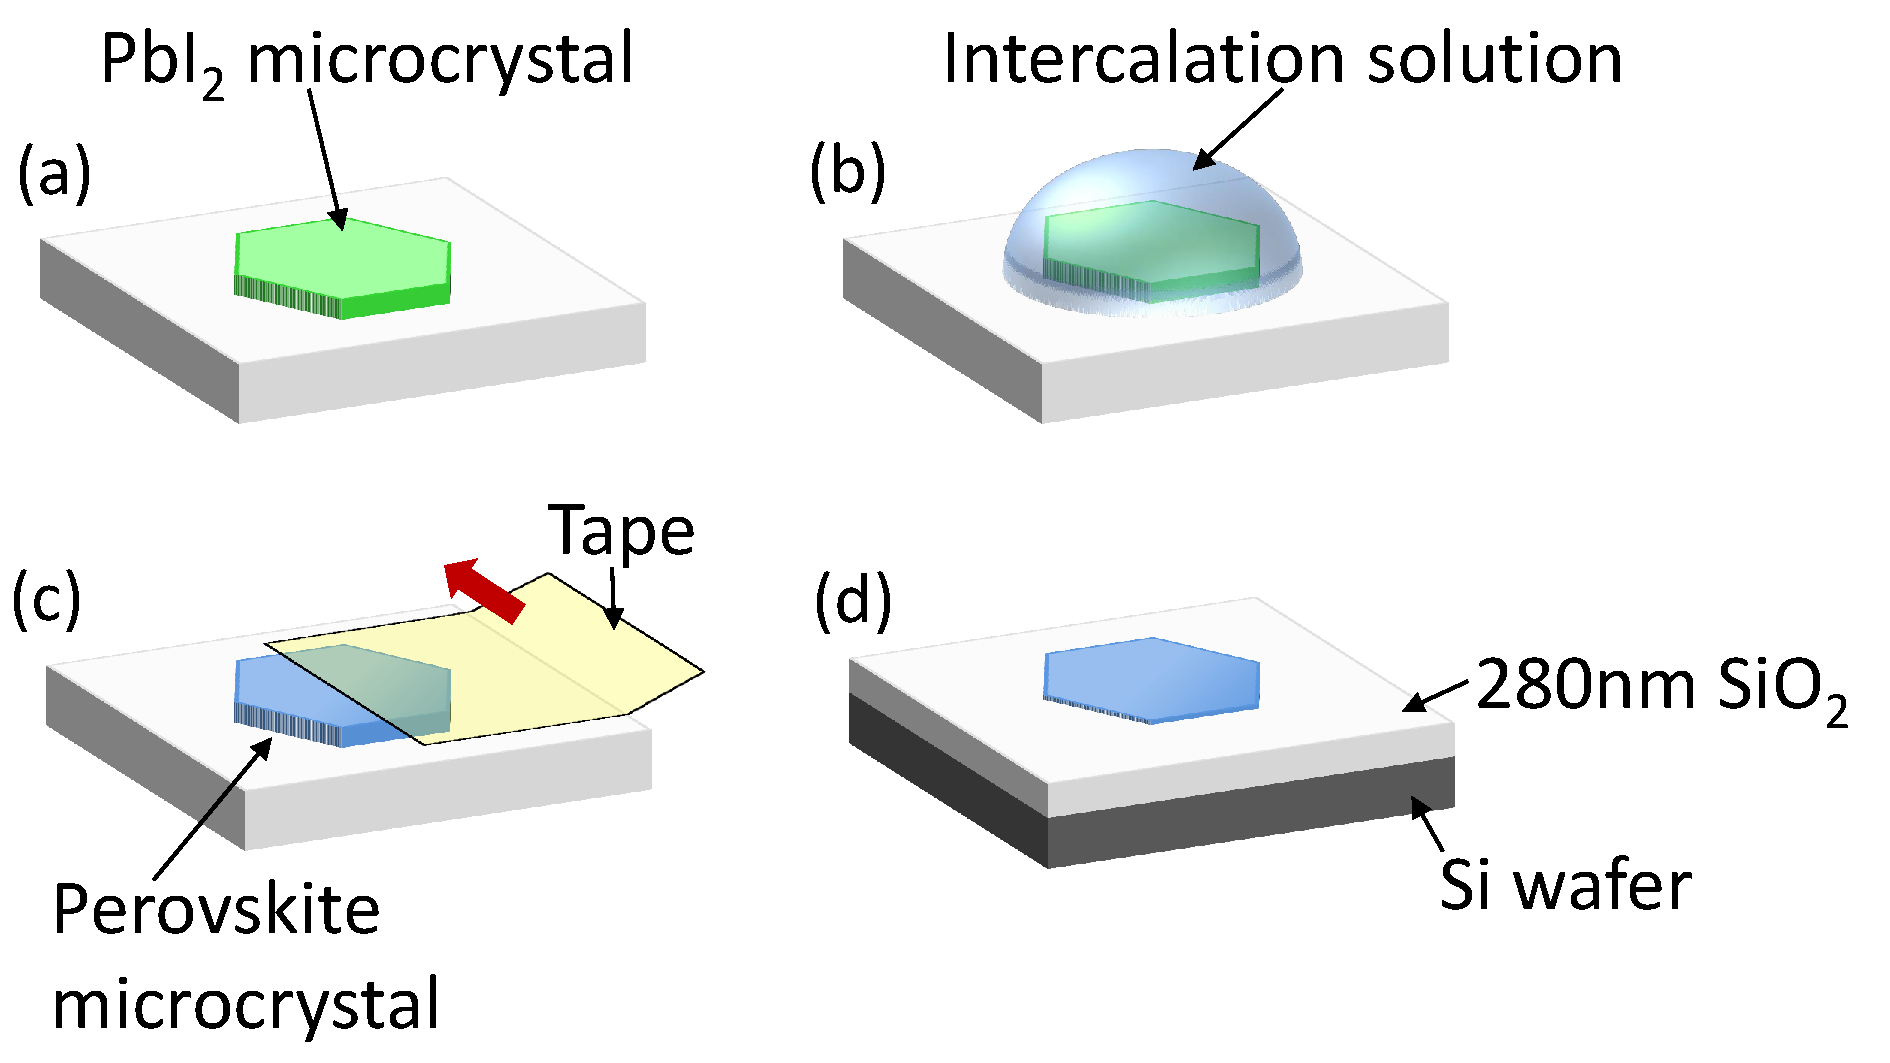
\includegraphics[width=0.7\textwidth]{Fig1}
\caption{Preparation of exfoliated perovskite samples.}
\label{5Fig1}
\end{figure}

\section{Exfoliated CHPI samples}
BF images of intercalated CHPI and C$_{12}$PI microcrystals at 20$\times$ magnification are shown in Fig.\,\ref{5Fig2}(a,b). Reflectivity spectra for such microcrystals shown an exciton resonance at $\sim500$nm indicating formation of the 2D MQW structure, with Fabry-Perot fringing due to the finite crystal thickness, typically $\sim1\,\mu$m. The top surfaces of crystals are rough as a result of etching by the intercalation solution, however such surfaces should adhere to the tape during exfoliation, and will therefore not be present in the measured samples. The exciton wavelength (grey dashed line) varies from literature values as a build up of strain in thick layer stacks can lead to structural distortions/rearrangements and thus change the exciton energy \cite{Saikumar2012, VijayaPrakash2009, Pradeesh2009b}. 
\begin{figure}[h!] 
\centering    
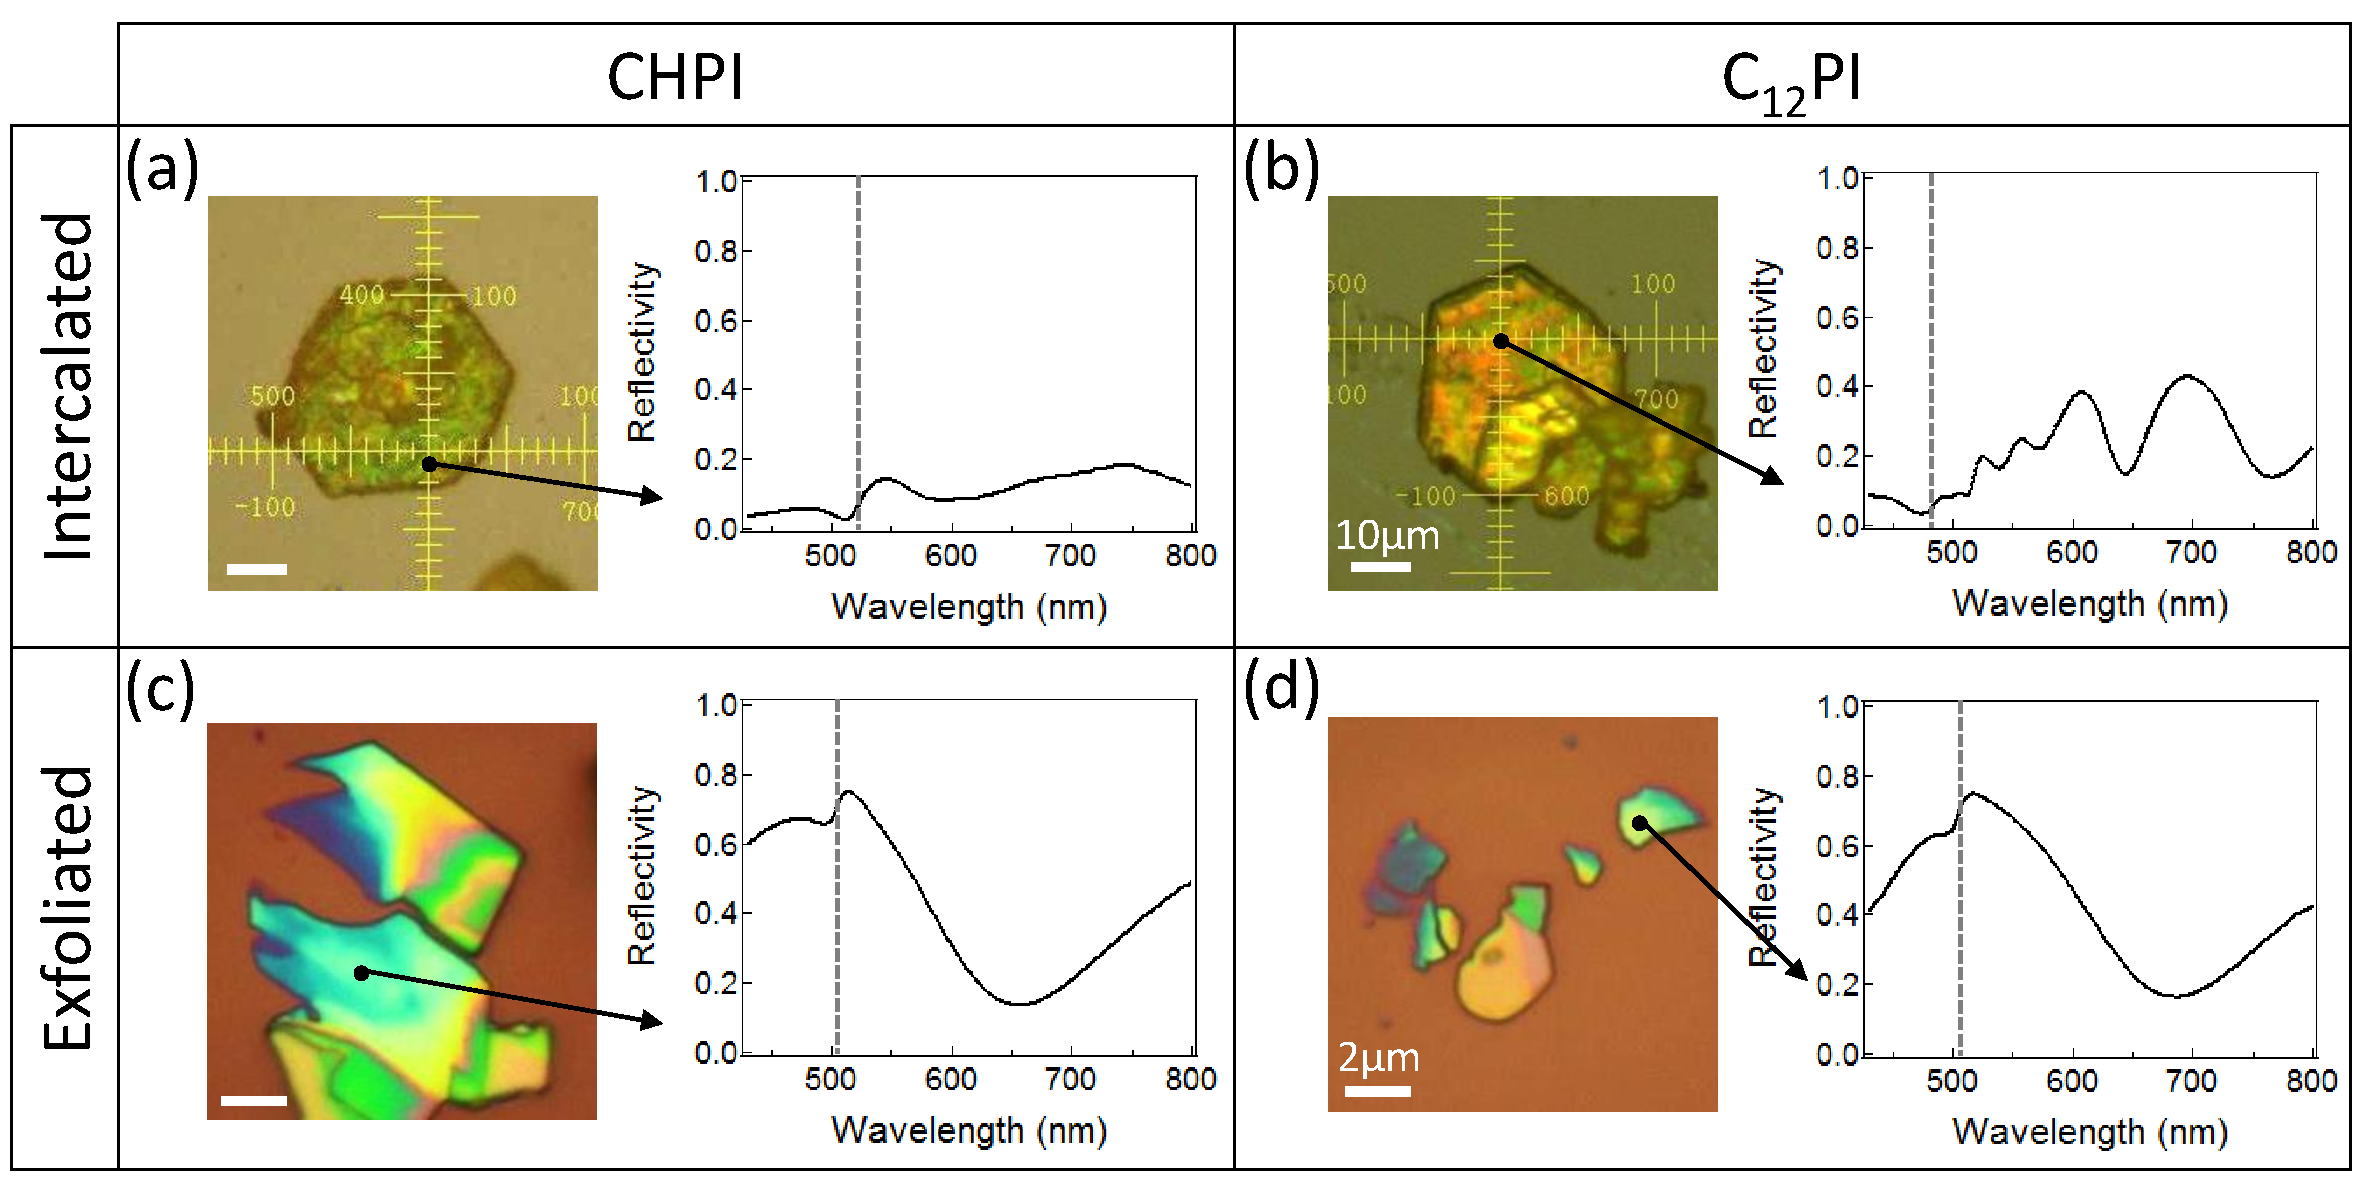
\includegraphics[width=\textwidth]{Fig2}
\caption[Intercalated and exfoliated perovskite microcrystals.]{Bright field images of intercalated (a) CHPI and (b) C$_{12}$PI microcrystals on glass at 20$\times$ magnification, and exfoliated (c) CHPI and (d) C$_{12}$PI flakes at 100$\times$ magnification. The reflectivity spectra of the areas indicated are shown on the right. Grey dashed lines indicate the wavelength of the exciton resonance.}
\label{5Fig2}
\end{figure}

BF images of exfoliated flakes of CHPI and C$_{12}$PI [Fig.\,\ref{5Fig2}(c,d)] show similar features. Although the crystals are fractured during the exfoliation process, we are able to obtain ultra-thin samples ($<20$\,nm) with lateral sizes $\sim1-10\,\mu$m. We observe excitonic resonances in both CHPI and C$_{12}$PI samples, however due to the bistability of C$_{12}$PI we use CHPI samples for further analysis.
\begin{figure}[h!]
\centering
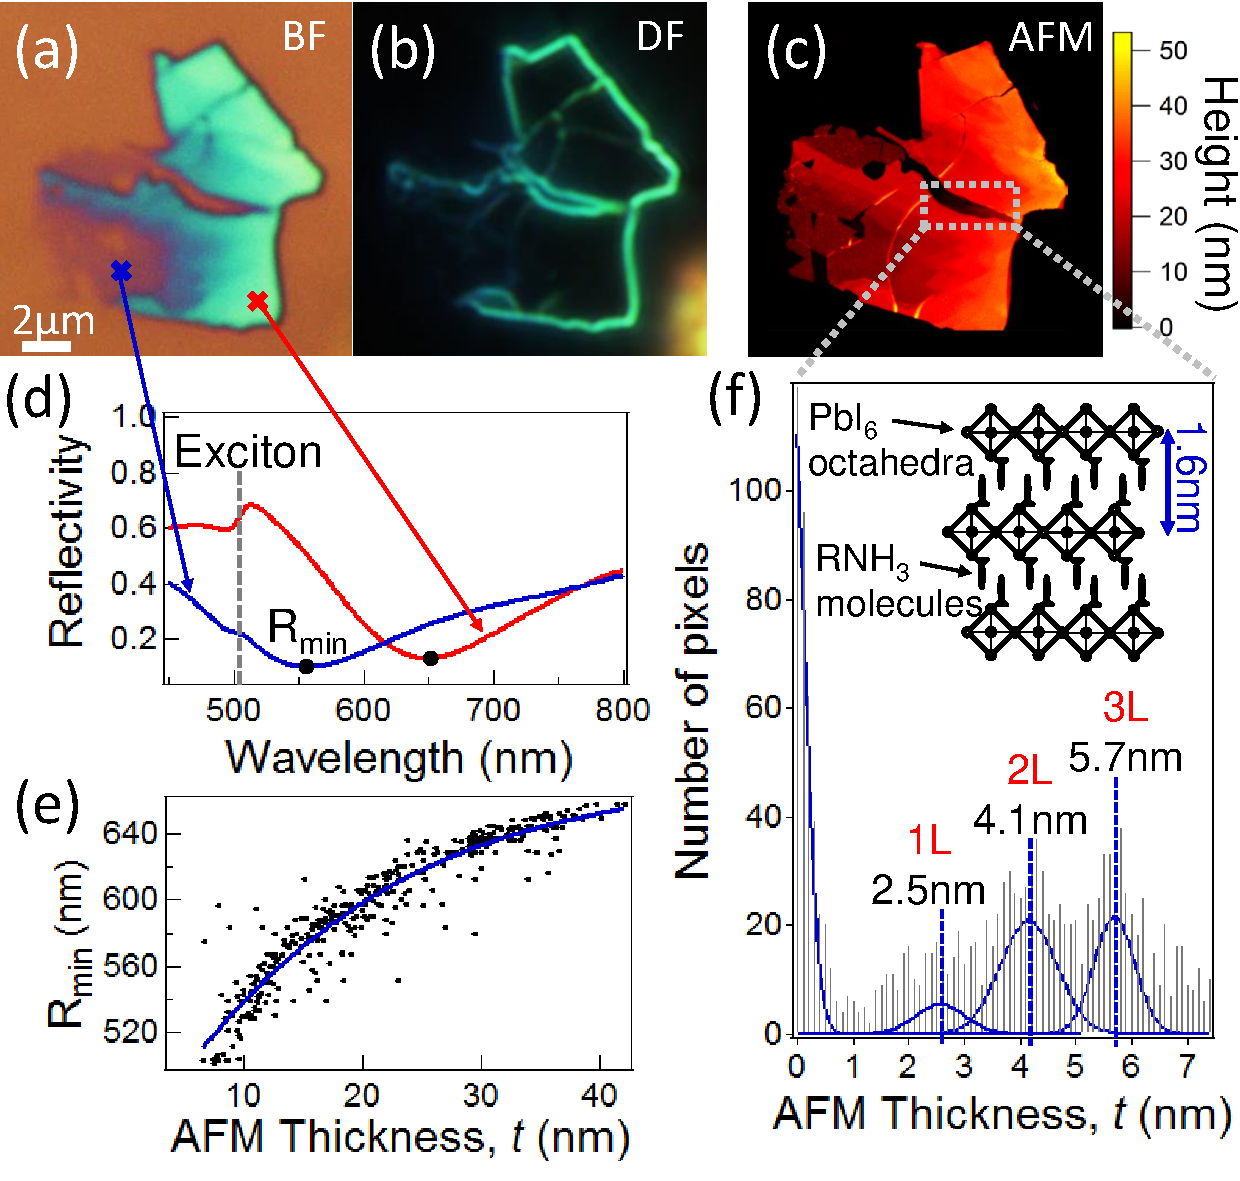
\includegraphics[width=0.8\textwidth]{Fig3}
\caption{Images in 100$\times$ magnification using (a) bright and (b) dark field on an exfoliated CHPI flake; (c) AFM image of the same area. (d) Reflectivity spectra of two regions on the flake. The exciton wavelength is indicated by the dashed line. (e) Relationship between the measured reflectivity minimum (labelled as $\textnormal{R}_\textnormal{min}$ in (d)) and AFM thickness. (f) Histogram of heights measured in the boxed area of (c). Multipeak fitting to the data (blue lines) gives an interlayer spacing of 1.6\,nm. The inset shows the structure of 2D PbI perovskites.}
\label{5Fig3}
\end{figure}

BF and DF reflection images of a typical CHPI flake are shown at 100$\times$ magnification in Figs.\,\ref{5Fig3}(a,b) respectively. The DF scattering seen from the edges and grain boundaries of the sample is typical for such crystals. The reflectivity spectra for these exfoliated samples [Fig.\,\ref{5Fig3}(d)] consist of an excitonic Fano resonance at $\lambda_{ex}\negmedspace\approx\negmedspace504$\,nm superimposed on a background of Fabry-Perot fringes. These fringes correspond to the colour of the crystal seen in BF, and come from the path difference experienced by light double passing through the flake. The oxide layer on the substrate is designed to maximize optical contrast for very thin layers, and while optimized for graphene, this 280\,nm \ce{SiO2}/Si system also works well for CHPI. By using this spectral information in conjunction with AFM measurements [Fig.\,\ref{5Fig3}(e)], we can correlate the position of Fabry-Perot fringes with thickness $t$. Thus it is then possible to spectroscopically determine the thickness of CHPI flakes.

A histogram of AFM heights in the boxed area of Fig.\,\ref{5Fig3}(c) shows three predominant thicknesses, which can be fit to Gaussians separated by steps of 1.6\,nm [Fig.\,\ref{5Fig3}(f)]. This interlayer spacing agrees well with X-ray diffraction measurements, where the periodicity was found to be 1.7-1.8\,nm \cite{Billing2006b, Pradeesh2009a}. Due to the presence of molecules adsorbed on the surface of the substrate, the initial step of 2.5\,nm is likely due to a monolayer, allowing us to label the three peaks as 1-, 2-, and 3-layer regions.  

Spectroscopic measurements of flake thickness require detailed knowledge of the CHPI refractive index, which is not well known. Instead we extract the required information from reflectivity data using the transfer matrix formulation \cite{Born1999}. In the wavelength range of interest (460\,-\,750\,nm), the dielectric function $\epsilon$ of 2D PbI perovskites can be modelled as the sum of a constant background and two Lorentzian oscillators: the exciton ($ex$) and an additional charge transfer ($CT$) transition at $\sim\negmedspace400$\,nm \cite{VijayaPrakash2009, Fujisawa2004, Fujisawa2005, Fujisawa2007, Mitzi1999a, Zhang2010}. Hence
\begin{equation}
\centering
\epsilon = \epsilon_1+i\epsilon_2+\frac{A_{ex}}{\lambda_{ex}^2-\lambda^2+i\Gamma_{ex}\lambda}+\frac{A_{CT}}{\lambda_{CT}^2-\lambda^2+i\Gamma_{CT}\lambda} ,
\label{CHPI_model}
\end{equation}
where $\epsilon_1, \epsilon_2$ are the background terms, while $A_i$ is the amplitude, $\lambda_i$ the wavelength, and $\Gamma_i$ the linewidth of oscillator $i$. The refractive index ($\tilde{n} = \sqrt{\epsilon}$) can then be used in the multilayer transfer matrix to calculate the expected reflectivity. The $CT$ peak, due to the charge transfer between organic and inorganic layers, is particular sensitive to disorder and the local dielectric environment, and depends on the precise spin coating conditions when comparable thin films are produced \cite{VijayaPrakash2009}. 

\begin{figure}[h!]
\centering
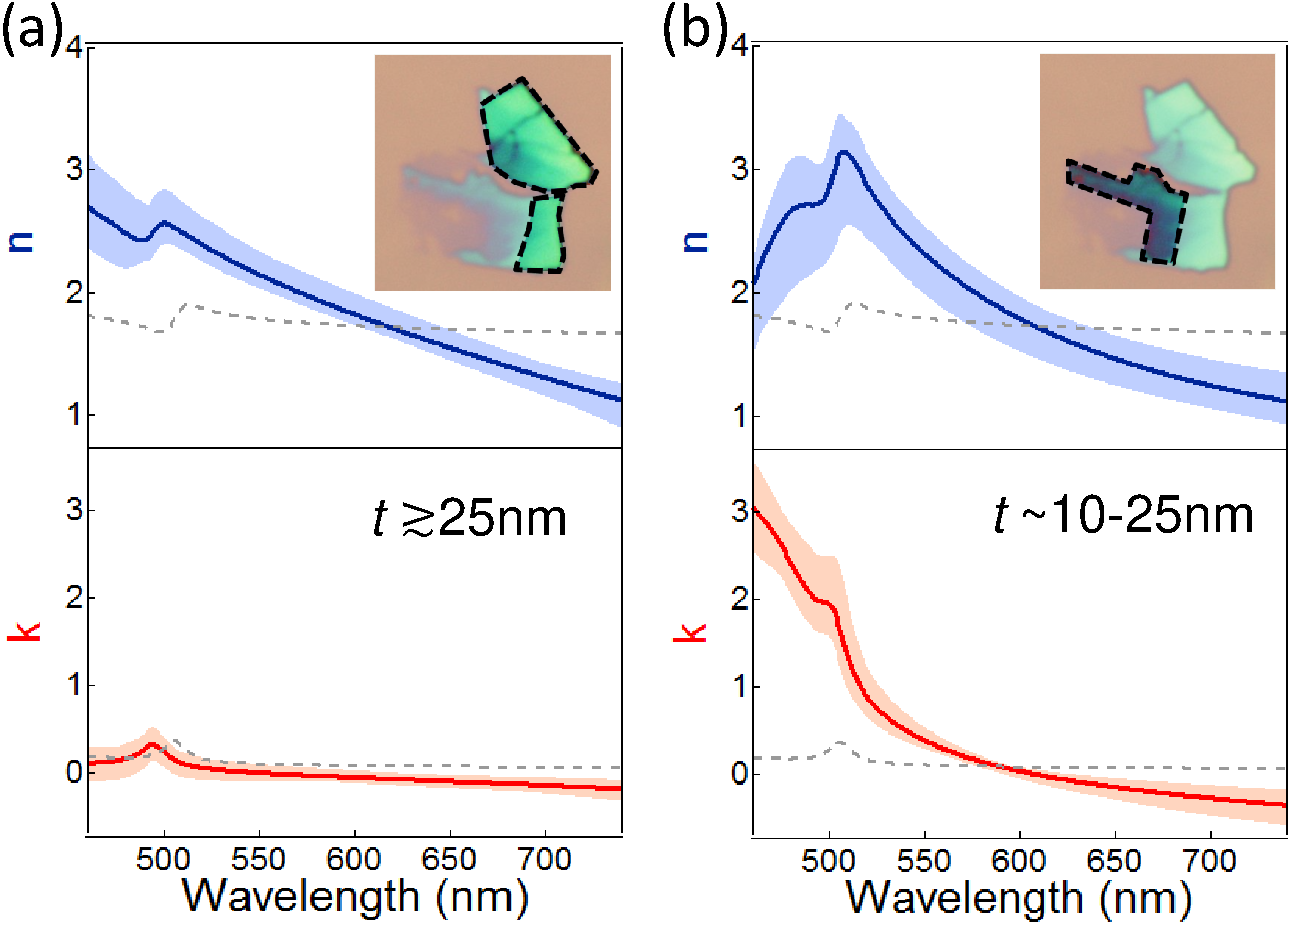
\includegraphics[width=0.8\textwidth]{Fig4}
\caption[Fitted complex refractive index of CHPI flakes for more than 200 pixels. Two regimes are found: (a) low absorption, occurring at positions of high thickness ($t\negmedspace\gtrsim\negmedspace25$\,nm), and (b) high absorption, at lower thickness ($t\negmedspace\sim\negmedspace10\negmedspace-\negmedspace25$\,nm).]{Fitted complex refractive index of CHPI flakes for more than 200 pixels. Two regimes are found: (a) low absorption, occurring at positions of high thickness ($t\negmedspace\gtrsim\negmedspace25$\,nm), and (b) high absorption, at lower thickness ($t\negmedspace\sim\negmedspace10\negmedspace-\negmedspace25$\,nm). The insets indicate typical areas where each regime is found. Shaded regions show the range of values extracted from the fit, and grey dotted lines represent the refractive index of a CHPI film ($t\negmedspace\sim\negmedspace60$\,nm) measured using ellipsometry.}
\label{5Fig4}
\end{figure}

The results of these refractive index fits for more than 200 spectra are shown in Fig.\,\ref{5Fig4}. The fitting works well for spectra that are not collected at the edges of the flake, therefore the thinnest areas are excluded. Within these regions, two main regimes of refractive index are observed. In both cases the background and exciton oscillator are relatively unchanged. For thicker areas of the sample ($t\negmedspace\gtrsim\negmedspace25$\,nm) a low-absorption regime is observed, where the $CT$ oscillator is mainly reflective. For thinner areas ($t\negmedspace\sim\negmedspace10\negmedspace-\negmedspace25$\,nm) a high-absorption regime is seen, where the $CT$ oscillator redshifts and becomes more optically active. As discussed below, the thickness range encompassed by the absorbing regime is correlated with a region of structural reconfiguration. This leads to a change in the energy states of the hybrid perovskite, and modifies the charge transfer between neighbouring organic and inorganic sheets. For comparison, the refractive index of a $t\negmedspace\sim\negmedspace60$\,nm film extracted from ellipsometry (grey dashed line) is also shown in Fig.\,\ref{5Fig4}. The film absorption ($k$) is closer to that of thicker flake areas, with a reduced contribution from the $CT$ oscillator in the refractive index. X-ray diffraction shows that while distinct layers are formed during spin coating, there is greater structural disorder in each layer when compared with intercalated \ce{PbI2} microcrystals \cite{Saikumar2012}. This interface mismatch can be responsible for a large range of charge transfer environments, leading to the reduced strength of the $CT$ resonance that we observe here.

\begin{figure}[h!]
\centering
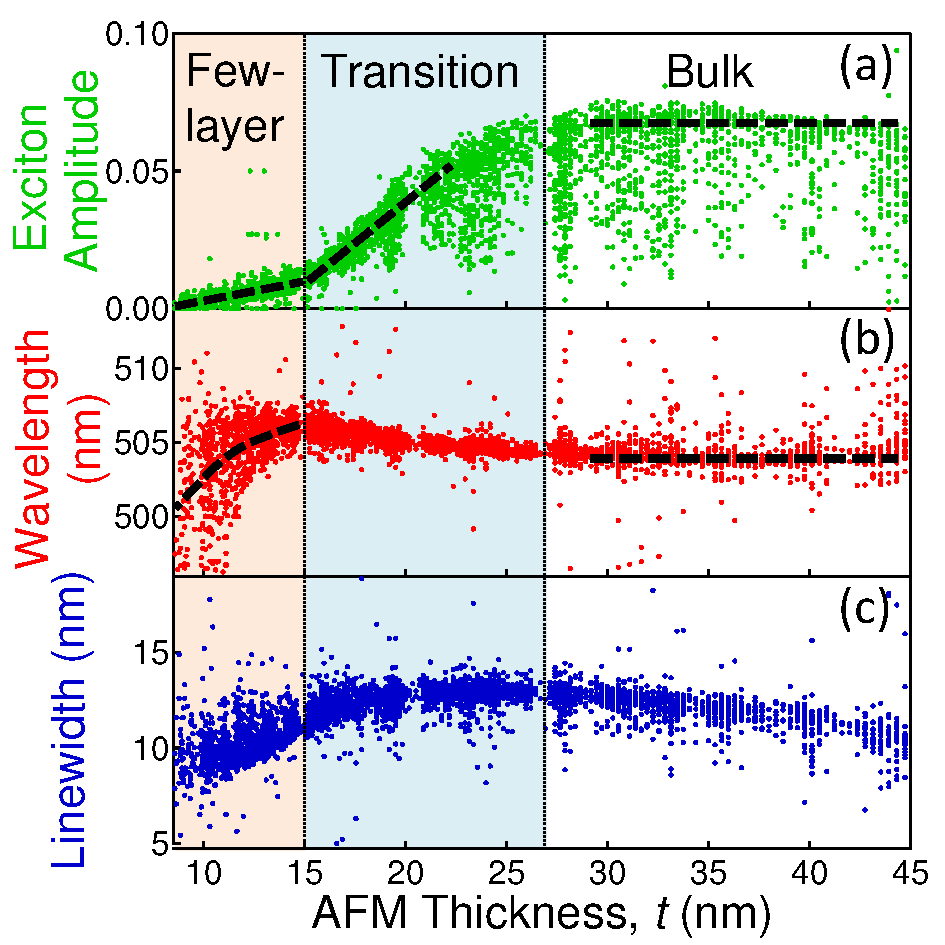
\includegraphics[width=0.8\textwidth]{Fig5}
\caption{Fitted exciton (a) amplitude, (b) wavelength, and (c) linewidth from reflectivity spectra (see Eq.\,\ref{R_fit}). Dashed lines are guides for the eye.}
\label{5Fig5}
\end{figure}

In reflectivity the exciton produces a Fano lineshape due to interference between its narrow resonance and the continuum background. On account of this complication, we extract information about exciton properties by describing $\Delta R = R_{\textnormal{CHPI}} - R_{substrate}$ as
\begin{equation}
\centering
\Delta R = R_{bkg} + A\frac{(\lambda - \lambda_{ex} + q\gamma)^2}{(\lambda - \lambda_{ex})^2 + \gamma^2} , 
\label{R_fit}
\end{equation}
where $R_{bkg}$ represents the continuum background with Fabry-Perot fringing; $A$, $\lambda_{ex}$ and $\gamma$ are the amplitude, wavelength, and linewidth of the exciton respectively, and the parameter $q$ describes the asymmetric shape of the Fano resonance. The results of the fit are shown in Fig.\,\ref{5Fig5} for positions across many flakes with different thicknesses. $A$, $\lambda_{ex}$ and $\gamma$ are equivalent to the corresponding terms in Eq.\,\ref{CHPI_model}, while $q$ represents the interference between the exciton, CT and background terms. Near the vicinity of the exciton the effects of the CT and background are not distinguished, therefore Eq.\,\ref{R_fit} allows us to focus exclusive on the exciton components, while Eq.\,\ref{CHPI_model} gives us the overall refractive index. Since the perovskite resembles a multilayer system, we find the exciton amplitude initially scales linearly with the number of layers as expected, before saturating at $t\negmedspace\approx\negmedspace27$\,nm (15 layers). The large variability of amplitudes at high thickness arises predominantly from spectra taken at edges of flakes. Linear extrapolation of our data indicates the exciton amplitude will drop to zero at $t\negmedspace\sim\negmedspace7$\,nm (3 layers). However layer-by-layer assembly of perovskite films has shown that linear increases in the exciton intensity occur only after the fourth layer, while two monolayers are required to observe room temperature exciton behaviour \cite{Matsui2002}. 

From Fig.\,\ref{5Fig5}, we identify 3 regions of interest. Firstly the `bulk' region ($t\negmedspace\gtrsim\negmedspace27$\,nm), where the exciton wavelength remains roughly constant; secondly the transition region ($t\negmedspace\sim\negmedspace15\negmedspace-\negmedspace27$\,nm), where the wavelength begins to redshift, while the linewidth reaches a maximum; and finally the few-layer region, where the wavelength blueshifts below the bulk limit, along with a decrease in the linewidth. This data helps us understand the changes happening at a structural level: disorder causes inhomogeneous broadening of the exciton resonance \cite{Baranovskii1993, Andreani1998, Kuznetsova2010}, while the exciton energy is directly related to the angle between \ce{PbI6} octahedra in the inorganic layers \cite{Pradeesh2009}. In `bulk' CHPI, the exciton has a wavelength of 504\,nm and a spectral width of $\approx\negmedspace10$\,nm. Close to the thickness transition region, the system is seen to become more disordered as the PbI sheets rearrange, becoming flatter and more strained. Finally at small $t$, the few-layer regime reveals how the layers relax and crumple again to reach the lowest energy configuration. Extrapolation of the fitted exciton wavelength to monolayer thickness (3\,nm) leads to a wavelength of $\sim\negmedspace495$\,nm, comparable to the value of $\sim\negmedspace490$\,nm reported for \ce{PbI2} thin films \cite{Iwasaki1978, Goto1987}. We were unable to spectroscopically probe areas with $t\negmedspace<\negmedspace8$\,nm (4 layers) as they lie on the edges of flakes, and are around 100\,nm in size. Since the lateral resolution of reflectivity measurements is $1\,\mu$m, these spectra are averaged with the much bigger signals from thicker areas. In order to achieve more sizeable monolayer regions, large-area samples are desirable for exfoliation, for instance using solution-grown single crystals. Exfoliating onto flexible polymer substrates may also improve our capability for attaining large monolayer regions as this can reduce fracture of crystals. However our measurements clearly show that these organic-inorganic hybrid perovskites change their electronic properties as the thickness is reduced, and this is connected to changes in the strain, disorder and layer structure.

\section{Conclusions}
In conclusion, we report the exfoliation of 2D organic-inorganic perovskites. Monolayers are observed, and the interlayer distance was found to be 1.6\,nm. As with other 2D materials, the thinnest regions (\textless8 layers) behave differently from the bulk material due to the influence of strain on the layer structure. We note however that the active excitonic layers are already electronically isolated in these hybrids, so changes in the band structure as observed in dichalcogenide systems are not expected. Instead, the effects seen are due to the re-organisation of organic molecules around the inorganic sheets. This suggests that pre-organisation of the intercalating molecules is key to controlling material structure at the monolayer scale, which may be accessible through chemical growth rather than exfoliation. This work suggests the potential to construct optoelectronic devices for monolayers of these hybrid materials, offering new routes to emission. 
